\documentclass[11pt,a4paper]{article}
\usepackage{mathpazo}
\usepackage{verbatim}

\usepackage{tikz}
\usetikzlibrary{intersections,calc,through,arrows.meta}
\tikzset {>=Stealth}

\usepackage{url}

\newtheorem{theorem}{Theorem}
\newtheorem{definition}{Definition}

\textwidth=15cm
\textheight=23cm
\topmargin=0pt
\headheight=0pt
\oddsidemargin=2em
\headsep=0pt
\parindent=0pt
\renewcommand{\baselinestretch}{1.15}
\setlength{\parskip}{0.3\baselineskip plus 1pt minus 1pt}

\newenvironment{form}[1]{%
\begin{displaymath}%
\renewcommand{\arraystretch}{#1}%
\begin{array}{lcl}}%
{\end{array}%
\end{displaymath}%
}

\begin{document}

\thispagestyle{empty}
\begin{center}
\textbf{\LARGE How to Guard a Museum}

\bigskip

\textbf{\Large Moti Ben-Ari\\\bigskip\url{http://www.weizmann.ac.il/sci-tea/benari/}}


\medskip
\end{center}


\begin{footnotesize}
\begin{center}
\copyright{}\  2021 by Moti Ben-Ari. 
\end{center}
This work is licensed under the Creative Commons Attribution-ShareAlike 3.0 Unported License. To view a copy of this license, visit \url{http://creativecommons.org/licenses/by-sa/3.0/} or send a letter to Creative Commons, 444 Castro Street, Suite 900, Mountain View, California, 94041, USA.

\end{footnotesize}

\bigskip

This document is based on Chapter~39 of Martin Aigner and Günter M. Ziegler. \textit{Proofs from THE BOOK (Fifth Edition)}. Springer-Verlag, Berlin Heidelberg, 2014. I have included many additional drawings and proofs.

\section{Introduction}
In 1973 Victor Klee asked how many guards are need to continually observe all the walls of a museum to ensure that no paintings are stolen. If the walls of the museum form a regular polygon or even a convex polygon, one guard is enough:

\begin{center}
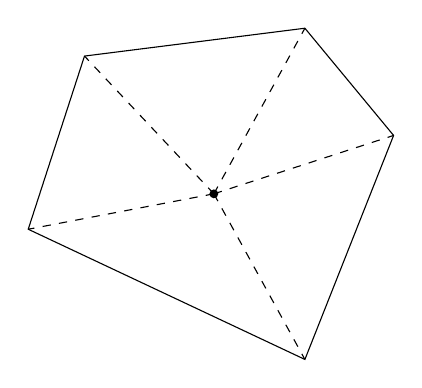
\begin{tikzpicture}[scale=.8]
\coordinate (O) at (0,0);
\fill (O) circle (2pt);
\foreach \x/\name/\n/\po in {0/a/A/right,.6/b/B/above,1.6/c/C/left,2.4/d/D/below left,3.9/e/E/below right} {
  \coordinate (\name) at ($(O)+(\x*72+18:3cm)$);
%  \fill (\name) circle (1.5pt);
%  \node[\po] at (\name) {$\n$};
\draw[dashed] (O) -- (\name);
}
\draw (a) -- (b) -- (c) -- (d) --(e) -- cycle;
\end{tikzpicture}
\end{center}

Consider now a museum with saw-toothed walls:

\begin{center}
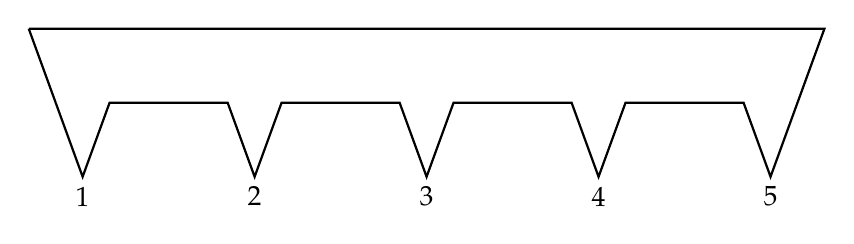
\begin{tikzpicture}[scale=1]
\coordinate (O) at (0,0);
\draw [thick] (O) -- (++110:1cm) coordinate (P);
\draw[thick] (O) --
  ++(-70:1cm) coordinate(A) node[below] {$1$} -- 
  ++(+70:1cm) -- ++(0:1.5cm) --
  ++(-70:1cm) coordinate(B) node[below] {$2$} -- 
  ++(+70:1cm) -- ++(0:1.5cm) --
  ++(-70:1cm) coordinate(C) node[below] {$3$}-- 
  ++(+70:1cm) -- ++(0:1.5cm) --
  ++(-70:1cm) coordinate(D) node[below] {$4$} -- 
  ++(+70:1cm) -- ++(0:1.5cm) --
  ++(-70:1cm) coordinate(E) node[below] {$5$} --
  ++(+70:2cm) -- (P);

\end{tikzpicture}
\end{center}

Verify by counting that the museum has $15$ walls.

\newpage

Let us shade the triangles formed by each tooth:

\begin{center}
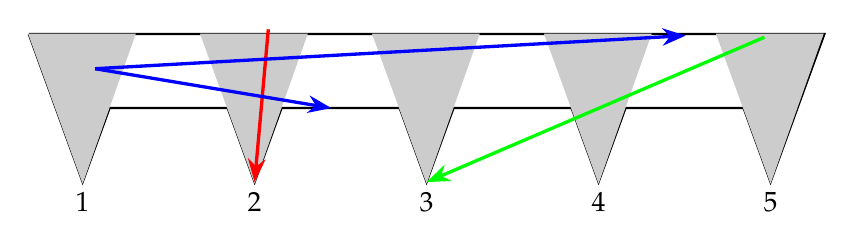
\begin{tikzpicture}[scale=1]
\coordinate (O) at (0,0);
\draw [thick] (O) -- (++110:1cm) coordinate (P);
\draw[thick] (O) --
  ++(-70:1cm) coordinate(A) node[below] {$1$} -- 
  ++(+70:1cm) -- ++(0:1.5cm) --
  ++(-70:1cm) coordinate(B) node[below] {$2$} -- 
  ++(+70:1cm) -- ++(0:1.5cm) --
  ++(-70:1cm) coordinate(C) node[below] {$3$}-- 
  ++(+70:1cm) -- ++(0:1.5cm) --
  ++(-70:1cm) coordinate(D) node[below] {$4$} -- 
  ++(+70:1cm) -- ++(0:1.5cm) --
  ++(-70:1cm) coordinate(E) node[below] {$5$} --
  ++(+70:2cm) -- (P);

\draw[fill,black!20!white] (A) -- ++(110:2cm) -- ++(0:1.35cm)-- cycle;
\draw[fill,black!20!white] (B) -- ++(110:2cm) -- ++(0:1.35cm)-- cycle;
\draw[fill,black!20!white] (C) -- ++(110:2cm) -- ++(0:1.35cm)-- cycle;
\draw[fill,black!20!white] (D) -- ++(110:2cm) -- ++(0:1.35cm)-- cycle;
\draw[fill,black!20!white] (E) -- ++(110:2cm) -- ++(0:1.35cm)-- cycle;

\draw[->,red,very thick] (2.7,1) -- (B);
\draw[->,very thick,green] (9,.9) -- (C);
\draw[->,very thick,blue] ($(O)+(.5,.5)$) -- ++(7.5,.42);
\draw[->,very thick,blue] ($(O)+(.5,.5)$) -- ++(3,-.5);
\end{tikzpicture}
\end{center}

A guard placed anywhere within one of the shaded triangles can observe all the walls of the triangle (red arrow). Furthermore, if the guard is placed near or at the top wall spanning the entire museum, she can observe all the horizontal walls (blue arrows). Clearly, $\frac{15}{3}=5$ guards are sufficient to observe all the walls of the museum. If the shaded triangles do not overlap, a guard in one shaded triangle will not be able to observe all the walls of another shaded triangle (green arrow), so $5$ guards are necessary.

This example can be generalized to $\frac{n}{3}$ teeth with $n$ walls, so we conclude that \emph{at least} $\frac{n}{3}$ guards are necessary. The following theorem claims that $\frac{n}{3}$ guards are sufficient.

\begin{theorem}\label{thm.guarded} Any museum with $n$ walls can be guarded by $\frac{n}{3}$ guards.\footnote{If $n$ is not divisible by $3$ the number of guards needed is $\lfloor \frac{n}{3}\rfloor$. For example, $4$ guards are sufficient for museums with $12, 13, 14$ walls since $\lfloor \frac{14}{3}\rfloor =\lfloor \frac{13}{3}\rfloor=\lfloor \frac{12}{3}\rfloor=4$. For simplicity we ignore this complication.}
\end{theorem}

Consider an arbitrary polygon, possibly a polygon with concave vertices. A vertex is \emph{convex} if its interior angle is less than $180^\circ$; a vertex is \emph{concave} if its interior angle is greater than $180^\circ$. In the polygon shown in the following diagram, vertex $1$ is convex and vertex $2$ is concave.

\begin{center}
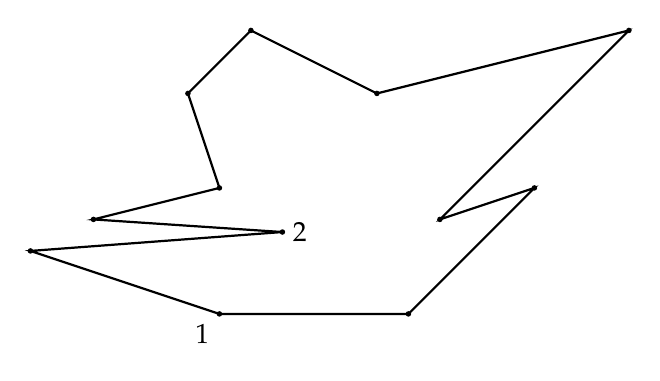
\begin{tikzpicture}[scale=.8]
\draw[thick]
  (0,0) coordinate (A) node[below left] {$1$} -- 
  ++(3,0) coordinate (B) --
  ++(2,2) coordinate (C) --
  ++(-1.5,-.5) coordinate (D) --
  ++(3,3) coordinate (E) -- 
  ++(-4,-1) coordinate (F) --
  ++(-2,1) coordinate (G) --
  ++(-1,-1) coordinate (H) --
  ++(.5,-1.5) coordinate (I) --
  ++(-2,-.5) coordinate (J) --
  ++(3,-.2) coordinate (K) node[right] {$2$} -- 
  ++(-4,-.3) coordinate (L) --
  cycle;
  
\foreach \point in {A,B,C,D,E,F,G,H,I,J,K,L}
  \fill (\point) circle(1.25pt);
\end{tikzpicture}
\end{center}

\begin{definition} A polygon is triangulated if \emph{non-intersecting diagonals} can be drawn such that the interior of the polygon is covered by triangles.
\end{definition}

\begin{theorem}
Any polygon can be triangulated.\label{thm.tri}
\end{theorem}

We defer the proof of Theorem~\ref{thm.tri}.

\begin{definition}
A polygon can be \emph{$3$-colored} if there is a map $c: V \mapsto \{\mathit{red},\mathit{blue},\mathit{green}\}$, such that the two vertices of an edge are assigned different colors.
\end{definition}

\begin{theorem}
A triangulated polygon can be $3$-colored.\label{thm.colored}
\end{theorem}

\textbf{Proof} By induction on the number of vertices. Clearly, a triangle can be $3$-colored. Consider a polygon with $n>3$ vertices. At least one diagonal must be drawn to triangulate the polygon. Choose some arbitrary diagonal $\overline{AB}$:

\begin{center}
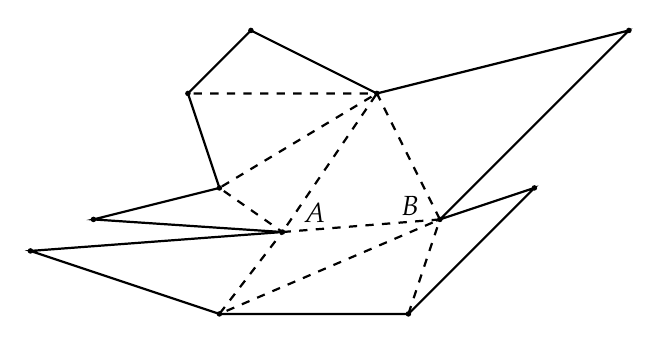
\begin{tikzpicture}[scale=.8]
\draw[thick]
  (0,0) coordinate (A) -- 
  ++(3,0) coordinate (B) --
  ++(2,2) coordinate (C) --
  ++(-1.5,-.5) coordinate (D) --
  ++(3,3) coordinate (E) -- 
  ++(-4,-1) coordinate (F) --
  ++(-2,1) coordinate (G) --
  ++(-1,-1) coordinate (H) --
  ++(.5,-1.5) coordinate (I) --
  ++(-2,-.5) coordinate (J) --
  ++(3,-.2) coordinate (K) -- 
  ++(-4,-.3) coordinate (L) --
  cycle;
  
\foreach \point in {A,B,C,D,E,F,G,H,I,J,K,L}
  \fill (\point) circle(1.25pt);

\node[above right,xshift=4pt] at (K) {$A$};
\node[above left,xshift=-4pt,yshift=-2pt] at (D) {$B$};

\draw[thick,dashed]
  (B) -- (D) -- (K) -- (F) -- (I) -- (K) -- (A) -- (D) -- (F) -- (H);
\end{tikzpicture}
\end{center}
and divide the polygon along this diagonal into two smaller polygons:
\begin{center}
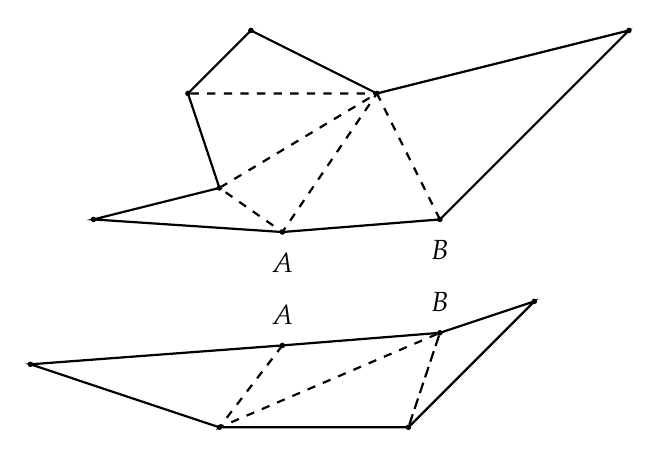
\begin{tikzpicture}[scale=.8]
\path
  (0,0) coordinate (A1) -- 
  ++(3,0) coordinate (B1) --
  ++(2,2) coordinate (C1) --
  ++(-1.5,-.5) coordinate (D1);
\draw[thick]
  (D1) --
  ++(3,3) coordinate (E1) -- 
  ++(-4,-1) coordinate (F1) --
  ++(-2,1) coordinate (G1) --
  ++(-1,-1) coordinate (H1) --
  ++(.5,-1.5) coordinate (I1) --
  ++(-2,-.5) coordinate (J1) --
  ++(3,-.2) coordinate (K1);
\path
  (K1) -- 
  ++(-4,-.3) coordinate (L1) --
  (A1);
  
\foreach \point in {D1,E1,F1,G1,H1,I1,J1,K1}
  \fill (\point) circle(1.25pt);

\node[below,yshift=-4pt] at (K1) {$A$};
\node[below,yshift=-4pt] at (D1) {$B$};

\draw[thick,dashed]
  (D1) -- (F1) -- (I1) -- (K1) -- (F1) -- (H1);
\draw[thick] (D1) -- (K1);


\begin{scope}[yshift=-1.8cm]

\draw[thick]
  (0,0) coordinate (A2) -- 
  ++(3,0) coordinate (B2) --
  ++(2,2) coordinate (C2) --
  ++(-1.5,-.5) coordinate (D2);
\path
  (D2) --
  ++(3,3) coordinate (E2) --
  ++(-4,-1) coordinate (F2) --
  ++(-2,1) coordinate (G2) --
  ++(-1,-1) coordinate (H2) --
  ++(.5,-1.5) coordinate (I2) --
  ++(-2,-.5) coordinate (J2) --
  ++(3,-.2) coordinate (K2);
\draw[thick]
  (K2) --
  ++(-4,-.3) coordinate (L2) --
  (A2);
  
\foreach \point in {A2,B2,C2,D2,K2,L2}
  \fill (\point) circle(1.25pt);
  
\node[above,yshift=4pt] at (K2) {$A$};
\node[above,yshift=4pt] at (D2) {$B$};

\draw[thick,dashed]
  (K2) -- (A2) -- (D2) -- (B2) -- (D2);
\draw[thick] (D2) -- (K2);

\end{scope}
\end{tikzpicture}
\end{center}

By induction, each of these smaller polygons can be $3$-colored:\begin{center}
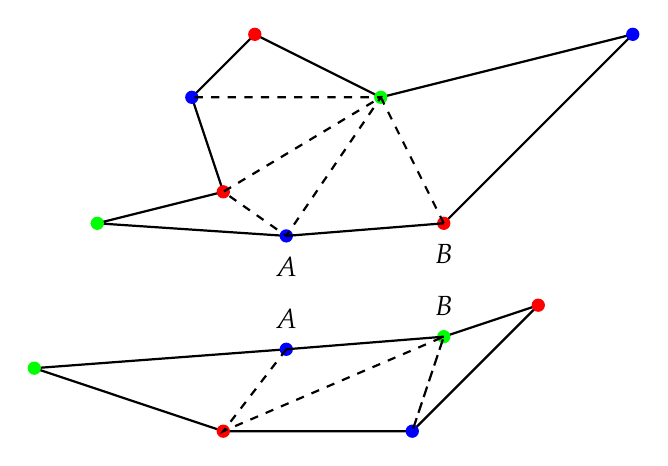
\begin{tikzpicture}[scale=.8]
\path
  (0,0) coordinate (A1) -- 
  ++(3,0) coordinate (B1) --
  ++(2,2) coordinate (C1) --
  ++(-1.5,-.5) coordinate (D1);
\draw[thick]
  (D1) --
  ++(3,3) coordinate (E1) -- 
  ++(-4,-1) coordinate (F1) --
  ++(-2,1) coordinate (G1) --
  ++(-1,-1) coordinate (H1) --
  ++(.5,-1.5) coordinate (I1) --
  ++(-2,-.5) coordinate (J1) --
  ++(3,-.2) coordinate (K1);
\path
  (K1) -- 
  ++(-4,-.3) coordinate (L1) --
  (A1);
  
\foreach \point/\color in {D1/red,E1/blue,F1/green,G1/red,H1/blue,I1/red,J1/green,K1/blue}
  \fill[color=\color] (\point) circle(3pt);

\draw[thick,dashed]
  (D1) -- (F1) -- (I1) -- (K1) -- (F1) -- (H1);
\draw[thick] (D1) -- (K1);

\node[below,yshift=-4pt] at (K1) {$A$};
\node[below,yshift=-4pt] at (D1) {$B$};

\begin{scope}[yshift=-1.8cm]

\draw[thick]
  (0,0) coordinate (A2) -- 
  ++(3,0) coordinate (B2) --
  ++(2,2) coordinate (C2) --
  ++(-1.5,-.5) coordinate (D2);
\path
  (D2) --
  ++(3,3) coordinate (E2) --
  ++(-4,-1) coordinate (F2) --
  ++(-2,1) coordinate (G2) --
  ++(-1,-1) coordinate (H2) --
  ++(.5,-1.5) coordinate (I2) --
  ++(-2,-.5) coordinate (J2) --
  ++(3,-.2) coordinate (K2);
\draw[thick]
  (K2) --
  ++(-4,-.3) coordinate (L2) --
  (A2);
  
\foreach \point/\color in {A2/red,B2/blue,C2/red,D2/green,K2/blue,L2/green}
  \fill[color=\color] (\point) circle(3pt);

\draw[thick,dashed]
  (K2) -- (A2) -- (D2) -- (B2) -- (D2);
\draw[thick] (D2) -- (K2);
\node[above,yshift=4pt] at (K2) {$A$};
\node[above,yshift=4pt] at (D2) {$B$};

\end{scope}
\end{tikzpicture}
\end{center}

Since the colors assigned are arbitrary, if different colors are assigned to $A,B$ in the two polygons, we can rename the colors in one of them so that the colors of $A,B$ are the same in both polygons. Here we exchange \emph{red} and \emph{green} in the lower polygon:

\begin{center}
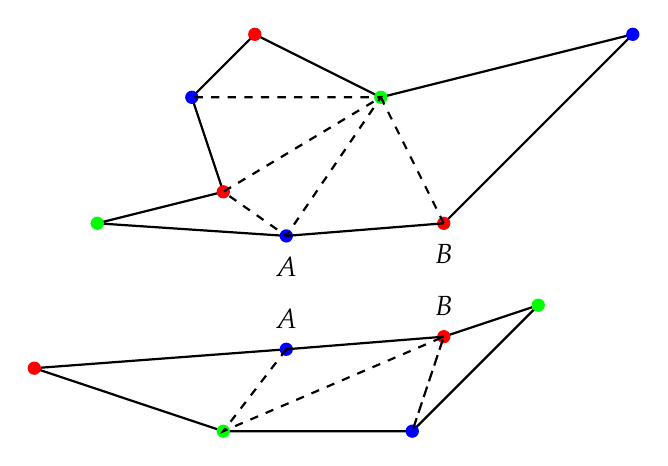
\begin{tikzpicture}[scale=.8]
\path
  (0,0) coordinate (A1) -- 
  ++(3,0) coordinate (B1) --
  ++(2,2) coordinate (C1) --
  ++(-1.5,-.5) coordinate (D1);
\draw[thick]
  (D1) --
  ++(3,3) coordinate (E1) -- 
  ++(-4,-1) coordinate (F1) --
  ++(-2,1) coordinate (G1) --
  ++(-1,-1) coordinate (H1) --
  ++(.5,-1.5) coordinate (I1) --
  ++(-2,-.5) coordinate (J1) --
  ++(3,-.2) coordinate (K1);
\path
  (K1) -- 
  ++(-4,-.3) coordinate (L1) --
  (A1);
  
\foreach \point/\color in {D1/red,E1/blue,F1/green,G1/red,H1/blue,I1/red,J1/green,K1/blue}
  \fill[color=\color] (\point) circle(3pt);
\node[below,yshift=-4pt] at (K1) {$A$};
\node[below,yshift=-4pt] at (D1) {$B$};

\draw[thick,dashed]
  (D1) -- (F1) -- (I1) -- (K1) -- (F1) -- (H1);
\draw[thick] (D1) -- (K1);

\begin{scope}[yshift=-1.8cm]

\draw[thick]
  (0,0) coordinate (A2) -- 
  ++(3,0) coordinate (B2) --
  ++(2,2) coordinate (C2) --
  ++(-1.5,-.5) coordinate (D2);
\path
  (D2) --
  ++(3,3) coordinate (E2) --
  ++(-4,-1) coordinate (F2) --
  ++(-2,1) coordinate (G2) --
  ++(-1,-1) coordinate (H2) --
  ++(.5,-1.5) coordinate (I2) --
  ++(-2,-.5) coordinate (J2) --
  ++(3,-.2) coordinate (K2);
\draw[thick]
  (K2) --
  ++(-4,-.3) coordinate (L2) --
  (A2);
  
\foreach \point/\color in {A2/green,B2/blue,C2/green,D2/red,K2/blue,L2/red}
  \fill[color=\color] (\point) circle(3pt);

\draw[thick,dashed]
  (K2) -- (A2) -- (D2) -- (B2) -- (D2);
\draw[thick] (D2) -- (K2);
\node[above,yshift=4pt] at (K2) {$A$};
\node[above,yshift=4pt] at (D2) {$B$};

\end{scope}
\end{tikzpicture}
\end{center}
Now ``paste'' the two polygons together to recover the original polygon with $n$ vertices. It will be $3$-colored:
\begin{center}
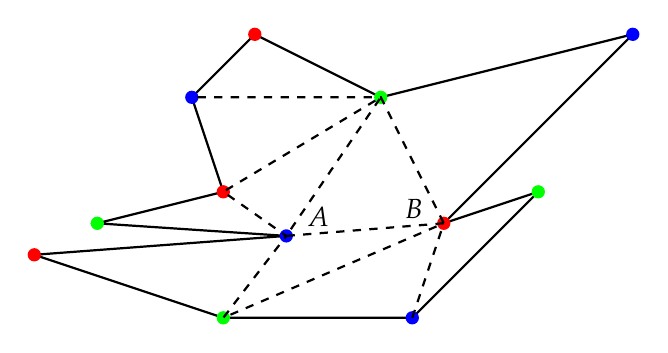
\begin{tikzpicture}[scale=.8]
\draw[thick]
  (0,0) coordinate (A) -- 
  ++(3,0) coordinate (B) --
  ++(2,2) coordinate (C) --
  ++(-1.5,-.5) coordinate (D) --
  ++(3,3) coordinate (E) -- 
  ++(-4,-1) coordinate (F) --
  ++(-2,1) coordinate (G) --
  ++(-1,-1) coordinate (H) --
  ++(.5,-1.5) coordinate (I) --
  ++(-2,-.5) coordinate (J) --
  ++(3,-.2) coordinate (K) -- 
  ++(-4,-.3) coordinate (L) --
  cycle;
  
\foreach \point/\color in {D/red,E/blue,F/green,G/red,H/blue,I/red,J/green,K/blue,A/green,B/blue,C/green,L/red}
  \fill[color=\color] (\point) circle(3pt);

\node[above right,xshift=4pt] at (K) {$A$};
\node[above left,xshift=-4pt,yshift=-2pt] at (D) {$B$};

\draw[thick,dashed]
  (B) -- (D) -- (K) -- (F) -- (I) -- (K) -- (A) -- (D) -- (F) -- (H);
\end{tikzpicture}
\end{center}

\textbf{Proof of Theorem~\ref{thm.guarded}}
By Theorem~\ref{thm.tri} the polygon can be triangulated and by Theorem~\ref{thm.colored} the polygon can be $3$-colored. All three vertices of each triangle in the triangulation must be colored by different colors in order to satisfy the condition of being $3$-colored. Since the polygon is $3$-colored, at least one color, say red, can appear at most $\frac{n}{3}$ times, and every triangle must have a vertex colored red. Station a guard at each red vertex; clearly, she can observe all the walls of the each triangle the vertex belongs to. Since the triangles of the triangulation include all the edges of the polygon, $\frac{n}{3}$ guards are sufficient to observe all the walls of the museum.

\newpage 

We now prove Theorem~\ref{thm.tri} that any polygon can be triangulated.

\begin{theorem}
The sum of the interior angles of a polygon with $n$ vertices is  $180^\circ(n-2)$.
\end{theorem}



\textbf{Proof}
First consider a convex polygon.
Denote its \emph{exterior angles} $\theta_i$:
\begin{center}
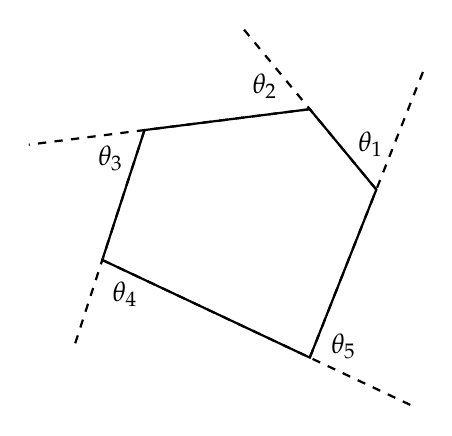
\begin{tikzpicture}[scale=.6]
\coordinate (O) at (0,0);
%\fill (O) circle (2pt);
\foreach \x/\name/\n/\po in {0/a/A/right,.6/b/B/above,1.6/c/C/left,2.4/d/D/below left,3.9/e/E/below right} {
  \coordinate (\name) at ($(O)+(\x*72+18:3cm)$);
%  \fill (\name) circle (1.5pt);
%  \node[\po] at (\name) {$\n$};
%\draw[dashed] (O) -- (\name);
}
\draw[thick] (a) -- (b) -- (c) -- (d) --(e) -- cycle;

\draw[thick,dashed] (a) 
  node[above,xshift=-2pt,yshift=8pt] {$\theta_1$} -- 
  ($(a)!2!(b)$);
\draw[thick,dashed] (b)
  node[above left,xshift=-8pt,yshift=0pt] {$\theta_2$} -- 
  ($(b)!1.7!(c)$);
\draw[thick,dashed] (c) 
  node[below left,xshift=-4pt,yshift=-2pt] {$\theta_3$} -- 
  ($(c)!1.7!(d)$);
\draw[thick,dashed] (d)
  node[below right,xshift=0pt,yshift=-4pt] {$\theta_4$} -- 
  ($(d)!1.5!(e)$);
\draw[thick,dashed] (e)
  node[right,xshift=4pt,yshift=4pt] {$\theta_5$} -- 
  ($(e)!1.7!(a)$);

\end{tikzpicture}
\end{center}
As you move one dashed line to the next, we complete a rotation around a circle so $\displaystyle\sum_1^n \theta_i = 360^\circ$. For each exterior angle $\theta_i$, denote its corresponding interior angle by $\phi_i$. Then:
\begin{form}{2}
\displaystyle\sum_1^n \theta_i =\displaystyle\sum_1^n (180^\circ-\phi_i)= 360^\circ\\
\displaystyle\sum_1^n \phi_i = n\cdot 180^\circ-360^\circ =180^\circ(n-2)\,.
\end{form}
Consider now adding a concave vertex:
\begin{center}
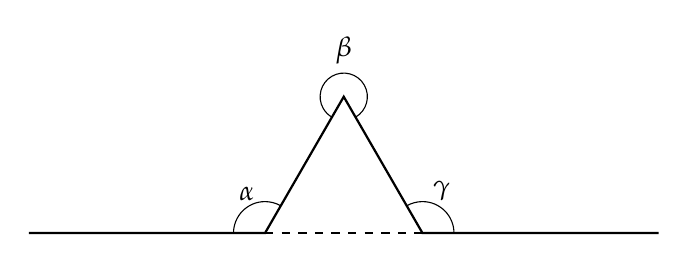
\begin{tikzpicture}
\draw[thick] (0,0) -- (3,0) coordinate (A) node[above left,yshift=8pt] {$\alpha$} -- ++(60:2) coordinate (B) node[above,yshift=8pt] {$\beta$} -- ++(-60:2) coordinate (C) node[above right,yshift=8pt] {$\gamma$}  -- ++(3,0);

\draw ($(A)+(-.4,0)$) arc(180:60:.4);
\draw ($(B)+(-60:.3)$) arc(-60:240:.3);
\draw ($(C)+(.4,0)$) arc(0:120:.4);

\draw[thick,dashed] (A) -- (C);
\end{tikzpicture}
\end{center}
There is a triangle formed by the two edges incident with the concave vertex and the dashed line connecting the other vertices of theses edges. By summing the angles of the triangle we get:
\begin{form}{1.2}
(180^\circ - \alpha) + (360^\circ - \beta) + (180^\circ - \gamma) = 180^\circ\\
\alpha + \beta + \gamma = 3\cdot 180^\circ\,.
\end{form}
The sum of the interior angles increases by $\alpha+\beta+\gamma$ while the number of vertices increases by three preserving the equation in the theorem:
\begin{form}{1.4}
\displaystyle\sum_1^n \phi_i + (\alpha + \beta + \gamma) &=& 180^\circ(n-2)+3\cdot 180^\circ\\
&=& 180^\circ((n+3)-2)\,.
\end{form}
\begin{theorem}\label{thm.convex}
There must be at least three convex vertices in a polygon.
\end{theorem}

\textbf{Proof} Let $k$ be the number of concave vertices, where the interior angle of each concave vertex is $180^\circ+\epsilon_i$, $\epsilon_i>0$. The sum of the interior angles of the \emph{concave} vertices is certainly less than or equal to the sum of the interior angles of \emph{all} the vertices:
\begin{form}{1.4}
k\cdot 180^\circ +\displaystyle\sum_{i=1}^{k}\epsilon_i &\leq& 180^\circ(n-2)\\
(k+2)\cdot 180^\circ +\displaystyle\sum_{i=1}^{k}\epsilon_i &\leq& n\cdot 180^\circ\\
(k+2)\cdot 180^\circ &<& n\cdot 180^\circ\\
k&<&n-2\,.
\end{form}
It follows that there must at least three vertices that are not concave, but convex.

\textbf{Proof of Theorem~\ref{thm.tri}} By induction on the number of vertices. For $n=3$ there is nothing to prove. Suppose that $n>3$; then by Theorem~\ref{thm.convex}, there must be a convex vertex $C$. Label its adjacent vertices by $B,D$. If $\overline{BD}$ is contained within the polygon, then it is a diagonal and the polygon can be split into the $\triangle BCD$ and another, smaller, polygon with $\overline{BD}$ as an edge. By the inductive hypothesis, the polygon can be triangulated and then glued to $\triangle BCD$, triangulating the original polygon. Otherwise, there must be concave vertex $F$ that is \emph{closest} to $C$. $\overline{CF}$ is a diagonal and splits the polygon into two smaller polygons. By the inductive hypothesis these can be triangulated and glued together.
\begin{center}
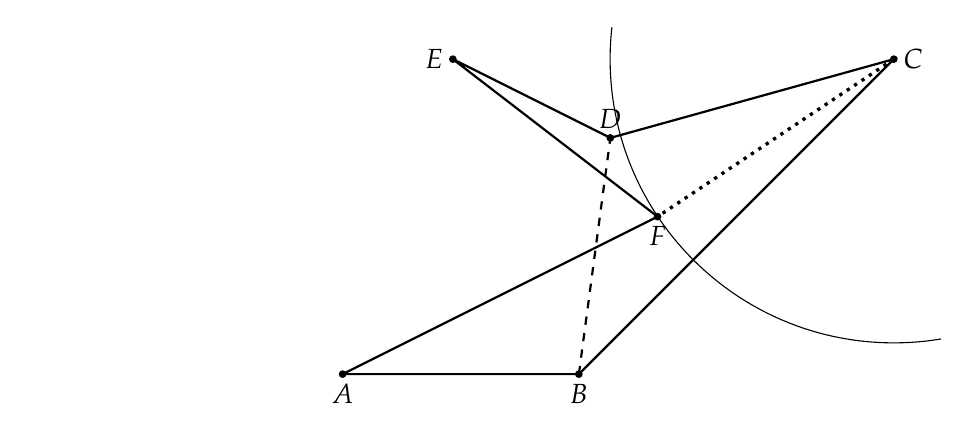
\begin{tikzpicture}[scale=2]
\clip (-2,-.2) rectangle (3.8,2.2);
\draw[thick]
  (0,0) coordinate (A) -- 
  ++(1.5,0) coordinate (B) --
  ++(2,2) coordinate (C) --
  ++(-1.8,-.5) coordinate (D) --
  ++(-1,.5) coordinate (E) --
  ++(1.3,-1) coordinate (F) --
  (A);
\draw[thick,dashed] (B) -- (D);
\draw[very thick,dotted] (C) -- (F);
\node [draw,circle through=(F)] at (C) {};
\foreach \point/\pos in {A/below,B/below,C/right,D/above,E/left,F/below}
  \fill (\point) circle(.7pt) node[\pos] {$\point$};
\end{tikzpicture}
\end{center}


\end{document}
